\chapter{Project: A Platform Game}\label{game}

\epigraphhead[30]{
\epigraph{\hspace*{-.1cm}\itshape``All reality is a game.''}%
{---Iain Banks, The Player of Games}
}\index{Banks, Ian}\index{project chapter}\index{simulation}

Much of my initial fascination with computers, like that of many nerdy kids, had to do with computer \index{game}games. I was drawn into the tiny simulated \index{world}worlds that I could manipulate and in which stories (sort of) unfolded—more, I suppose, because of the way I projected my \index{imagination}imagination into them than because of the possibilities they actually offered.

I don't wish a \index{career}career in game programming on anyone. Much like the \index{music}music industry, the discrepancy between the number of eager young people wanting to work in it and the actual demand for such people creates a rather unhealthy environment. But writing games for fun is amusing.\index{jump-and-run game}\index{dimensions}

This chapter will walk through the implementation of a small \index{platform game}platform game. Platform games (or ``jump and run'' games) are games that expect the \index{player}player to move a figure through a \index{world}world, which is usually two-dimensional and viewed from the side, while jumping over and onto things.

\section{The game}\index{minimalism}\index{Palef, Thomas}\index{Dark Blue (game)}

Our \index{game}game will be roughly based on \href{http://www.lessmilk.com/games/10}{Dark Blue} (\emph{www.lessmilk.com\slash games\slash 10}) by Thomas Palef. I chose that game because it is both entertaining and minimalist and because it can be built without too much \index{code}code. It looks like this:

\vskip 1.5ex
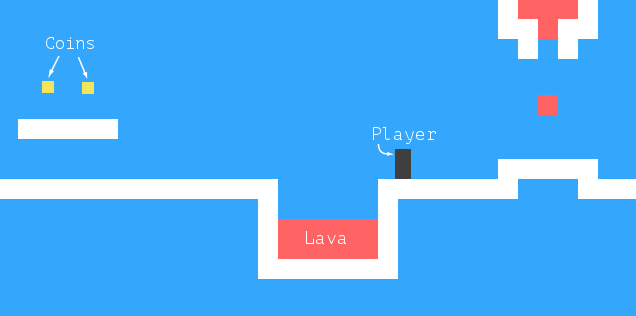
\includegraphics[width=10cm]{img/darkblue.png}
\vskip 1.5ex\index{coin}\index{lava}

The dark \index{box}box represents the \index{player}player, whose task is to collect the yellow boxes (coins) while avoiding the red stuff (lava). A \index{level}level is completed when all coins have been collected.\index{keyboard}\index{jumping}

The player can walk around with the left and right arrow keys and can jump with the up arrow. Jumping is a specialty of this game character. It can reach several times its own height and can change direction in midair. This may not be entirely realistic, but it helps give the player the feeling of being in direct control of the on-screen \index{avatar}avatar.\index{fractional number}\index{discretization}\index{artificial life}\index{electronic life}

The \index{game}game consists of a static \index{background}background, laid out like a \index{grid}grid, with the moving elements overlaid on that background. Each field on the grid is either empty, solid, or \index{lava}lava. The moving elements are the player, coins, and certain pieces of lava. The positions of these elements are not constrained to the grid—their coordinates may be fractional, allowing smooth \index{motion}motion.

\section{The technology}\index{event handling}\index{keyboard}\index{DOM!graphics}

We will use the \index{browser}browser DOM to display the game, and we'll read user input by handling key events.\index{rectangle}\index{background (CSS)}\index{position (CSS)}\index{graphics}

The screen- and keyboard-related code is only a small part of the work we need to do to build this \index{game}game. Since everything looks like colored \index{box}boxes, drawing is uncomplicated: we create DOM elements and use styling to give them a background color, size, and position.\index{table (HTML tag)}

We can represent the background as a table since it is an unchanging \index{grid}grid of squares. The free-moving elements can be overlaid using absolutely positioned elements.\index{performance}\index{DOM!graphics}

In games and other programs that should animate \index{graphics}graphics and respond to user \index{input}input without noticeable delay, \index{efficiency}efficiency is important. Although the DOM was not originally designed for high-performance graphics, it is actually better at this than you would expect. You saw some \index{animation}animations in \hyperref[dom.animation]{Chapter 14}. On a modern machine, a simple game like this performs well, even if we don't worry about \index{optimization}optimization very much.\index{canvas}\index{DOM!graphics}

In the \hyperref[canvas]{next chapter}, we will explore another \index{browser}browser technology, the \lstinline`<canvas>` tag, which provides a more traditional way to draw graphics, working in terms of shapes and \index{pixel}pixels rather than DOM elements.

\section{Levels}\index{dimensions}

We'll want a human-readable, human-editable way to specify levels. Since it is okay for everything to start out on a grid, we could use big strings in which each character represents an element—either a part of the background grid or a moving element.

The plan for a small level might look like this:

\begin{lstlisting}
let simpleLevelPlan = `
......................
..#................#..
..#..............=.#..
..#.........o.o....#..
..#.@......#####...#..
..#####............#..
......#++++++++++++#..
......##############..
......................`;
\end{lstlisting}
\noindent\index{level}

Periods are empty space, hash (\lstinline`#`) characters are walls, and plus signs are lava. The \index{player}player's starting position is the \index{at sign}at sign (\lstinline`@`). Every O character is a coin, and the equal sign (\lstinline`=`) at the top is a block of lava that moves back and forth horizontally.\index{bouncing}

We'll support two additional kinds of moving \index{lava}lava: the pipe character (\lstinline`|`) creates vertically moving blobs, and \lstinline`v` indicates \emph{dripping} lava—vertically moving lava that doesn't bounce back and forth but only moves down, jumping back to its start position when it hits the floor.

A whole \index{game}game consists of multiple \index{level}levels that the \index{player}player must complete. A level is completed when all \index{coin}coins have been collected. If the player touches \index{lava}lava, the current level is restored to its starting position, and the player may try again.

\label{game.level}\section{Reading a level}\index{Level class}

The following \index{class}class stores a \index{level}level object. Its argument should be the string that defines the level.

\begin{lstlisting}
class Level {
  constructor(plan) {
    let rows = plan.trim().split("\n").map(l => [...l]);
    this.height = rows.length;
    this.width = rows[0].length;
    this.startActors = [];

    this.rows = rows.map((row, y) => {
      return row.map((ch, x) => {
        let type = levelChars[ch];
        if (typeof type == "string") return type;
        this.startActors.push(
          type.create(new Vec(x, y), ch));
        return "empty";
      });
    });
  }
}
\end{lstlisting}
\noindent\index{trim method}\index{split method}\index{whitespace!trimming}

The \lstinline`trim` method is used to remove whitespace at the start and end of the plan string. This allows our example plan to start with a newline so that all the lines are directly below each other. The remaining string is split on \index{newline character}newline characters, and each line is spread into an array, producing arrays of characters.\index{array!as matrix}

So \lstinline`rows` holds an array of arrays of characters, the rows of the plan. We can derive the level's width and height from these. But we must still separate the moving elements from the background grid. We'll call moving elements \emph{actors}. They'll be stored in an array of objects. The background will be an array of arrays of strings, holding field types such as \lstinline`"empty"`, \lstinline`"wall"`, or \lstinline`"lava"`.\index{map method}

To create these arrays, we map over the rows and then over their content. Remember that \lstinline`map` passes the array index as a second argument to the mapping function, which tells us the x- and y-coordinates of a given character. Positions in the game will be stored as pairs of coordinates, with the top left being 0,0 and each background square being 1 unit high and wide.\index{static method}

To interpret the characters in the plan, the \lstinline`Level` constructor uses the \lstinline`levelChars` object, which maps background elements to strings and actor characters to classes. When \lstinline`type` is an actor class, its static \lstinline`create` method is used to create an object, which is added to \lstinline`startActors`, and the mapping function returns \lstinline`"empty"` for this background square.\index{Vec class}

The position of the actor is stored as a \lstinline`Vec` object. This is a two-dimensional vector, an object with \lstinline`x` and \lstinline`y` properties, as seen in the exercises of \hyperref[object.exercise_vector]{Chapter 6}.\index{state!in!objects}

As the game runs, actors will end up in different places or even disappear entirely (as coins do when collected). We'll use a \lstinline`State` class to track the state of a running game.

\begin{lstlisting}
class State {
  constructor(level, actors, status) {
    this.level = level;
    this.actors = actors;
    this.status = status;
  }

  static start(level) {
    return new State(level, level.startActors, "playing");
  }

  get player() {
    return this.actors.find(a => a.type == "player");
  }
}
\end{lstlisting}
\noindent

The \lstinline`status` property will switch to \lstinline`"lost"` or \lstinline`"won"` when the game has ended.

This is again a persistent data structure—updating the game state creates a new state and leaves the old one intact.

\section{Actors}\index{actor}\index{Vec class}\index{interface!object}

Actor objects represent the current position and state of a given moving element in our game. All actor objects conform to the same interface. Their \lstinline`pos` property holds the coordinates of the element's top-left corner, and their \lstinline`size` property holds its size.

Then they have an \lstinline`update` method, which is used to compute their new state and position after a given time step. It simulates the thing the actor does—moving in response to the arrow keys for the player and bouncing back and forth for the lava—and returns a new, updated actor object.

A \lstinline`type` property contains a string that identifies the type of the actor—\lstinline`"player"`, \lstinline`"coin"`, or \lstinline`"lava"`. This is useful when drawing the game—the look of the rectangle drawn for an actor is based on its type.

Actor classes have a static \lstinline`create` method that is used by the \lstinline`Level` constructor to create an actor from a character in the level plan. It is given the coordinates of the character and the character itself, which is needed because the \lstinline`Lava` class handles several different characters.

\label{game.vector}This is the \lstinline`Vec` class that we'll use for our two-dimensional values, such as the position and size of actors.

\begin{lstlisting}
class Vec {
  constructor(x, y) {
    this.x = x; this.y = y;
  }
  plus(other) {
    return new Vec(this.x + other.x, this.y + other.y);
  }
  times(factor) {
    return new Vec(this.x * factor, this.y * factor);
  }
}
\end{lstlisting}
\noindent\index{times method}\index{multiplication}

The \lstinline`times` method scales a vector by a given number. It will be useful when we need to multiply a speed vector by a time interval to get the distance traveled during that time.

The different types of actors get their own classes since their behavior is very different. Let's define these classes. We'll get to their \lstinline`update` methods later.\index{simulation}\index{Player class}

The player class has a property \lstinline`speed` that stores its current speed to simulate momentum and gravity.

\begin{lstlisting}
class Player {
  constructor(pos, speed) {
    this.pos = pos;
    this.speed = speed;
  }

  get type() { return "player"; }

  static create(pos) {
    return new Player(pos.plus(new Vec(0, -0.5)),
                      new Vec(0, 0));
  }
}

Player.prototype.size = new Vec(0.8, 1.5);
\end{lstlisting}
\noindent

Because a player is one-and-a-half squares high, its initial position is set to be half a square above the position where the \lstinline`@` character appeared. This way, its bottom aligns with the bottom of the square it appeared in.

The \lstinline`size` property is the same for all instances of \lstinline`Player`, so we store it on the prototype rather than on the instances themselves. We could have used a \index{getter}getter like \lstinline`type`, but that would create and return a new \lstinline`Vec` object every time the property is read, which would be wasteful. (Strings, being \index{immutable}immutable, don't have to be re-created every time they are evaluated.)\index{Lava class}\index{bouncing}

When constructing a \lstinline`Lava` actor, we need to initialize the object differently depending on the character it is based on. Dynamic lava moves along at its current speed until it hits an obstacle. At that point, if it has a \lstinline`reset` property, it will jump back to its start position (dripping). If it does not, it will invert its speed and continue in the other direction (bouncing).

The \lstinline`create` method looks at the character that the \lstinline`Level` constructor passes and creates the appropriate lava actor.

\begin{lstlisting}
class Lava {
  constructor(pos, speed, reset) {
    this.pos = pos;
    this.speed = speed;
    this.reset = reset;
  }

  get type() { return "lava"; }

  static create(pos, ch) {
    if (ch == "=") {
      return new Lava(pos, new Vec(2, 0));
    } else if (ch == "|") {
      return new Lava(pos, new Vec(0, 2));
    } else if (ch == "v") {
      return new Lava(pos, new Vec(0, 3), pos);
    }
  }
}

Lava.prototype.size = new Vec(1, 1);
\end{lstlisting}
\noindent\index{Coin class}\index{animation}

\lstinline`Coin` actors are relatively simple. They mostly just sit in their place. But to liven up the game a little, they are given a ``wobble'', a slight vertical back-and-forth motion. To track this, a coin object stores a base position as well as a \lstinline`wobble` property that tracks the \index{phase}phase of the bouncing motion. Together, these determine the coin's actual position (stored in the \lstinline`pos` property).

\begin{lstlisting}
class Coin {
  constructor(pos, basePos, wobble) {
    this.pos = pos;
    this.basePos = basePos;
    this.wobble = wobble;
  }

  get type() { return "coin"; }

  static create(pos) {
    let basePos = pos.plus(new Vec(0.2, 0.1));
    return new Coin(basePos, basePos,
                    Math.random() * Math.PI * 2);
  }
}

Coin.prototype.size = new Vec(0.6, 0.6);
\end{lstlisting}
\noindent\index{Math.random function}\index{random number}\index{Math.sin function}\index{sine}\index{wave}

In \hyperref[dom.sin_cos]{Chapter 14}, we saw that \lstinline`Math.sin` gives us the y-coordinate of a point on a circle. That coordinate goes back and forth in a smooth waveform as we move along the circle, which makes the sine function useful for modeling a wavy motion.\index{pi}

To avoid a situation where all coins move up and down synchronously, the starting phase of each coin is randomized. The \emph{\index{phase}phase} of \lstinline`Math.sin`'s wave, the width of a wave it produces, is 2π. We multiply the value returned by \lstinline`Math.random` by that number to give the coin a random starting position on the wave.\index{map}\index{object!as map}

We can now define the \lstinline`levelChars` object that maps plan characters to either background grid types or actor classes.

\begin{lstlisting}
const levelChars = {
  ".": "empty", "#": "wall", "+": "lava",
  "@": Player, "o": Coin,
  "=": Lava, "|": Lava, "v": Lava
};
\end{lstlisting}
\noindent

That gives us all the parts needed to create a \lstinline`Level` instance.

\begin{lstlisting}
let simpleLevel = new Level(simpleLevelPlan);
console.log(`${simpleLevel.width} by ${simpleLevel.height}`);
// → 22 by 9
\end{lstlisting}
\noindent

The task ahead is to display such levels on the screen and to model time and motion inside them.

\section{Encapsulation as a burden}\index{programming style}\index{program size}\index{complexity}

Most of the code in this chapter does not worry about \index{encapsulation}encapsulation very much for two reasons. First, encapsulation takes extra effort. It makes programs bigger and requires additional concepts and interfaces to be introduced. Since there is only so much code you can throw at a reader before their eyes glaze over, I've made an effort to keep the program small.\index{interface!design}

Second, the various elements in this game are so closely tied together that if the behavior of one of them changed, it is unlikely that any of the others would be able to stay the same. Interfaces between the elements would end up encoding a lot of assumptions about the way the game works. This makes them a lot less effective—whenever you change one part of the system, you still have to worry about the way it impacts the other parts because their interfaces wouldn't cover the new situation.

Some \emph{\index{cutting point}cutting points} in a system lend themselves well to separation through rigorous interfaces, but others don't. Trying to encapsulate something that isn't a suitable boundary is a sure way to waste a lot of energy. When you are making this mistake, you'll usually notice that your interfaces are getting awkwardly large and detailed and that they need to be changed often, as the program evolves.\index{graphics}\index{encapsulation}\index{graphics}

There is one thing that we \emph{will} encapsulate, and that is the \index{drawing}drawing subsystem. The reason for this is that we'll \index{display}display the same game in a different way in the \hyperref[canvas.canvasdisplay]{next chapter}. By putting the drawing behind an interface, we can load the same game program there and plug in a new display \index{module}module.

\label{game.domdisplay}\section{Drawing}\index{DOMDisplay class}\index{DOM!graphics}

The encapsulation of the \index{drawing}drawing code is done by defining a \emph{\index{display}display} object, which displays a given \index{level}level and state. The display type we define in this chapter is called \lstinline`DOMDisplay` because it uses DOM elements to show the level.\index{style attribute}\index{CSS}

We'll be using a style sheet to set the actual colors and other fixed properties of the elements that make up the game. It would also be possible to directly assign to the elements' \lstinline`style` property when we create them, but that would produce more verbose programs.\index{class attribute}

The following helper function provides a succinct way to create an element and give it some attributes and child nodes:

\begin{lstlisting}
function elt(name, attrs, ...children) {
  let dom = document.createElement(name);
  for (let attr of Object.keys(attrs)) {
    dom.setAttribute(attr, attrs[attr]);
  }
  for (let child of children) {
    dom.appendChild(child);
  }
  return dom;
}
\end{lstlisting}
\noindent

A display is created by giving it a parent element to which it should append itself and a \index{level}level object.

\begin{lstlisting}
class DOMDisplay {
  constructor(parent, level) {
    this.dom = elt("div", {class: "game"}, drawGrid(level));
    this.actorLayer = null;
    parent.appendChild(this.dom);
  }

  clear() { this.dom.remove(); }
}
\end{lstlisting}
\noindent\index{level}

The level's \index{background}background grid, which never changes, is drawn once. Actors are redrawn every time the display is updated with a given state. The \lstinline`actorLayer` property will be used to track the element that holds the actors so that they can be easily removed and replaced.\index{scaling}\index{DOMDisplay class}

Our \index{coordinates}coordinates and sizes are tracked in \index{grid}grid units, where a size or distance of 1 means one grid block. When setting \index{pixel}pixel sizes, we will have to scale these coordinates up—everything in the game would be ridiculously small at a single pixel per square. The \lstinline`scale` constant gives the number of pixels that a single unit takes up on the screen.

\begin{lstlisting}
const scale = 20;

function drawGrid(level) {
  return elt("table", {
    class: "background",
    style: `width: ${level.width * scale}px`
  }, ...level.rows.map(row =>
    elt("tr", {style: `height: ${scale}px`},
        ...row.map(type => elt("td", {class: type})))
  ));
}
\end{lstlisting}
\noindent\index{table (HTML tag)}\index{tr (HTML tag)}\index{td (HTML tag)}\index{spread operator}

As mentioned, the background is drawn as a \lstinline`<table>` element. This nicely corresponds to the structure of the \lstinline`rows` property of the level—each row of the grid is turned into a table row (\lstinline`<tr>` element). The strings in the grid are used as class names for the table cell (\lstinline`<td>`) elements. The spread (triple dot) operator is used to pass arrays of child nodes to \lstinline`elt` as separate arguments.

\label{game.game_css}The following \index{CSS}CSS makes the table look like the background we want:

\begin{lstlisting}
.background    { background: rgb(52, 166, 251);
                 table-layout: fixed;
                 border-spacing: 0;              }
.background td { padding: 0;                     }
.lava          { background: rgb(255, 100, 100); }
.wall          { background: white;              }
\end{lstlisting}
\noindent\index{padding (CSS)}

Some of these (\lstinline`table-layout`, \lstinline`border-spacing`, and \lstinline`padding`) are used to suppress unwanted default behavior. We don't want the layout of the \index{table}table to depend upon the contents of its cells, and we don't want space between the \index{table}table cells or padding inside them.\index{background (CSS)}\index{rgb (CSS)}\index{CSS}

The \lstinline`background` rule sets the background color. CSS allows colors to be specified both as words (\lstinline`white`) or with a format such as \lstinline`rgb(R, G, B)`, where the red, green, and blue components of the color are separated into three numbers from 0 to 255. So, in \lstinline`rgb(52, 166, 251)`, the red component is 52, green is 166, and blue is 251. Since the blue component is the largest, the resulting color will be bluish. You can see that in the \lstinline`.lava` rule, the first number (red) is the largest.\index{DOM!graphics}

We draw each \index{actor}actor by creating a DOM element for it and setting that element's position and size based on the actor's properties. The values have to be multiplied by \lstinline`scale` to go from game units to pixels.

\begin{lstlisting}
function drawActors(actors) {
  return elt("div", {}, ...actors.map(actor => {
    let rect = elt("div", {class: `actor ${actor.type}`});
    rect.style.width = `${actor.size.x * scale}px`;
    rect.style.height = `${actor.size.y * scale}px`;
    rect.style.left = `${actor.pos.x * scale}px`;
    rect.style.top = `${actor.pos.y * scale}px`;
    return rect;
  }));
}
\end{lstlisting}
\noindent\index{position (CSS)}\index{class attribute}

To give an element more than one class, we separate the class names by spaces. In the \index{CSS}CSS code shown next, the \lstinline`actor` class gives the actors their absolute position. Their type name is used as an extra class to give them a color. We don't have to define the \lstinline`lava` class again because we're reusing the class for the lava grid squares we defined earlier.

\begin{lstlisting}
.actor  { position: absolute;            }
.coin   { background: rgb(241, 229, 89); }
.player { background: rgb(64, 64, 64);   }
\end{lstlisting}
\noindent\index{graphics}\index{optimization}\index{efficiency}\index{state!of application}\index{DOM!graphics}

The \lstinline`syncState` method is used to make the display show a given state. It first removes the old actor graphics, if any, and then redraws the actors in their new positions. It may be tempting to try to reuse the DOM elements for actors, but to make that work, we would need a lot of additional bookkeeping to associate actors with DOM elements and to make sure we remove elements when their actors vanish. Since there will typically be only a handful of actors in the game, redrawing all of them is not expensive.

\begin{lstlisting}
DOMDisplay.prototype.syncState = function(state) {
  if (this.actorLayer) this.actorLayer.remove();
  this.actorLayer = drawActors(state.actors);
  this.dom.appendChild(this.actorLayer);
  this.dom.className = `game ${state.status}`;
  this.scrollPlayerIntoView(state);
};
\end{lstlisting}
\noindent\index{level}\index{class attribute}

By adding the level's current status as a class name to the wrapper, we can style the player actor slightly differently when the game is won or lost by adding a \index{CSS}CSS rule that takes effect only when the player has an \index{ancestor element}ancestor element with a given class.

\begin{lstlisting}
.lost .player {
  background: rgb(160, 64, 64);
}
.won .player {
  box-shadow: -4px -7px 8px white, 4px -7px 8px white;
}
\end{lstlisting}
\noindent\index{player}\index{box shadow (CSS)}

After touching \index{lava}lava, the player's color turns dark red, suggesting scorching. When the last coin has been collected, we add two blurred white shadows—one to the top left and one to the top right—to create a white halo effect.\index{position (CSS)}\index{max-width (CSS)}\index{overflow (CSS)}\index{max-height (CSS)}\index{viewport}\index{scrolling}\index{DOM!graphics}

\label{game.viewport}We can't assume that the level always fits in the \emph{viewport}—the element into which we draw the game. That is why the \lstinline`scrollPlayerIntoView` call is needed. It ensures that if the level is protruding outside the viewport, we scroll that viewport to make sure the player is near its center. The following \index{CSS}CSS gives the game's wrapping DOM element a maximum size and ensures that anything that sticks out of the element's box is not visible. We also give it a relative position so that the actors inside it are positioned relative to the level's top-left corner.

\begin{lstlisting}
.game {
  overflow: hidden;
  max-width: 600px;
  max-height: 450px;
  position: relative;
}
\end{lstlisting}
\noindent\index{scrolling}

In the \lstinline`scrollPlayerIntoView` method, we find the player's position and update the wrapping element's scroll position. We change the scroll position by manipulating that element's \lstinline`scrollLeft` and \lstinline`scrollTop` properties when the player is too close to the edge.

\begin{lstlisting}
DOMDisplay.prototype.scrollPlayerIntoView = function(state) {
  let width = this.dom.clientWidth;
  let height = this.dom.clientHeight;
  let margin = width / 3;

  // The viewport
  let left = this.dom.scrollLeft, right = left + width;
  let top = this.dom.scrollTop, bottom = top + height;

  let player = state.player;
  let center = player.pos.plus(player.size.times(0.5))
                         .times(scale);

  if (center.x < left + margin) {
    this.dom.scrollLeft = center.x - margin;
  } else if (center.x > right - margin) {
    this.dom.scrollLeft = center.x + margin - width;
  }
  if (center.y < top + margin) {
    this.dom.scrollTop = center.y - margin;
  } else if (center.y > bottom - margin) {
    this.dom.scrollTop = center.y + margin - height;
  }
};
\end{lstlisting}
\noindent\index{center}\index{coordinates}\index{readability}

The way the player's center is found shows how the methods on our \lstinline`Vec` type allow computations with objects to be written in a relatively readable way. To find the actor's center, we add its position (its top-left corner) and half its size. That is the center in level coordinates, but we need it in pixel coordinates, so we then multiply the resulting vector by our display scale.\index{validation}

Next, a series of checks verifies that the player position isn't outside of the allowed range. Note that sometimes this will set nonsense scroll coordinates that are below zero or beyond the element's scrollable area. This is okay—the DOM will constrain them to acceptable values. Setting \lstinline`scrollLeft` to -10 will cause it to become 0.

It would have been slightly simpler to always try to scroll the player to the center of the \index{viewport}viewport. But this creates a rather jarring effect. As you are jumping, the view will constantly shift up and down. It is more pleasant to have a ``neutral'' area in the middle of the screen where you can move around without causing any scrolling.\index{game!screenshot}

We are now able to display our tiny level.

\begin{lstlisting}
<link rel="stylesheet" href="css/game.css">

<script>
  let simpleLevel = new Level(simpleLevelPlan);
  let display = new DOMDisplay(document.body, simpleLevel);
  display.syncState(State.start(simpleLevel));
</script>
\end{lstlisting}
\noindent

\vskip 1.5ex
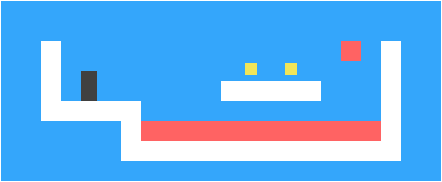
\includegraphics[width=7cm]{img/game_simpleLevel.png}
\vskip 1.5ex\index{link (HTML tag)}\index{CSS}

The \lstinline`<link>` tag, when used with \lstinline`rel="stylesheet"`, is a way to load a CSS file into a page. The file \lstinline`game.css` contains the styles necessary for our game.

\section{Motion and collision}\index{physics}\index{animation!platform game}

Now we're at the point where we can start adding motion—the most interesting aspect of the game. The basic approach, taken by most games like this, is to split \index{time}time into small steps and, for each step, move the actors by a distance corresponding to their speed multiplied by the size of the time step. We'll measure time in seconds, so speeds are expressed in units per second.\index{obstacle}\index{collision detection}

Moving things is easy. The difficult part is dealing with the interactions between the elements. When the player hits a wall or floor, they should not simply move through it. The game must notice when a given motion causes an object to hit another object and respond accordingly. For walls, the motion must be stopped. When hitting a coin, it must be collected. When touching lava, the game should be lost.

Solving this for the general case is a big task. You can find libraries, usually called \emph{\index{physics engine}physics engines}, that simulate interaction between physical objects in two or three \index{dimensions}dimensions. We'll take a more modest approach in this chapter, handling only collisions between rectangular objects and handling them in a rather simplistic way.\index{bouncing}\index{collision detection}\index{animation!platform game}

Before moving the \index{player}player or a block of \index{lava}lava, we test whether the motion would take it inside of a wall. If it does, we simply cancel the motion altogether. The response to such a collision depends on the type of actor—the player will stop, whereas a lava block will bounce back.\index{discretization}

This approach requires our \index{time}time steps to be rather small since it will cause motion to stop before the objects actually touch. If the time steps (and thus the motion steps) are too big, the player would end up hovering a noticeable distance above the ground. Another approach, arguably better but more complicated, would be to find the exact collision spot and move there. We will take the simple approach and hide its problems by ensuring the animation proceeds in small steps.\index{obstacle}\index{touches method}\index{collision detection}

\label{game.touches}This method tells us whether a \index{rectangle}rectangle (specified by a position and a size) touches a grid element of the given type.

\begin{lstlisting}
Level.prototype.touches = function(pos, size, type) {
  var xStart = Math.floor(pos.x);
  var xEnd = Math.ceil(pos.x + size.x);
  var yStart = Math.floor(pos.y);
  var yEnd = Math.ceil(pos.y + size.y);

  for (var y = yStart; y < yEnd; y++) {
    for (var x = xStart; x < xEnd; x++) {
      let isOutside = x < 0 || x >= this.width ||
                      y < 0 || y >= this.height;
      let here = isOutside ? "wall" : this.rows[y][x];
      if (here == type) return true;
    }
  }
  return false;
};
\end{lstlisting}
\noindent\index{Math.floor function}\index{Math.ceil function}

The method computes the set of grid squares that the body \index{overlap}overlaps with by using \lstinline`Math.floor` and \lstinline`Math.ceil` on its \index{coordinates}coordinates. Remember that \index{grid}grid squares are 1 by 1 units in size. By \index{rounding}rounding the sides of a box up and down, we get the range of \index{background}background squares that the box touches.

\vskip 1.5ex
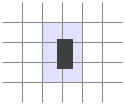
\includegraphics[width=3cm]{img/generated/game-grid.pdf}
\vskip 1.5ex

We loop over the block of \index{grid}grid squares found by \index{rounding}rounding the \index{coordinates}coordinates and return \lstinline`true` when a matching square is found. Squares outside of the level are always treated as \lstinline`"wall"` to ensure that the player can't leave the world and that we won't accidentally try to read outside of the bounds of our \lstinline`rows` array.

The state \lstinline`update` method uses \lstinline`touches` to figure out whether the player is touching lava.

\begin{lstlisting}
State.prototype.update = function(time, keys) {
  let actors = this.actors
    .map(actor => actor.update(time, this, keys));
  let newState = new State(this.level, actors, this.status);

  if (newState.status != "playing") return newState;

  let player = newState.player;
  if (this.level.touches(player.pos, player.size, "lava")) {
    return new State(this.level, actors, "lost");
  }

  for (let actor of actors) {
    if (actor != player && overlap(actor, player)) {
      newState = actor.collide(newState);
    }
  }
  return newState;
};
\end{lstlisting}
\noindent

The method is passed a time step and a data structure that tells it which keys are being held down. The first thing it does is call the \lstinline`update` method on all actors, producing an array of updated actors. The actors also get the time step, the keys, and the state, so that they can base their update on those. Only the player will actually read keys, since that's the only actor that's controlled by the keyboard.

If the game is already over, no further processing has to be done (the game can't be won after being lost, or vice versa). Otherwise, the method tests whether the player is touching background lava. If so, the game is lost, and we're done. Finally, if the game really is still going on, it sees whether any other actors overlap the player.

Overlap between actors is detected with the \lstinline`overlap` function. It takes two actor objects and returns true when they touch—which is the case when they overlap both along the x-axis and along the y-axis.

\begin{lstlisting}
function overlap(actor1, actor2) {
  return actor1.pos.x + actor1.size.x > actor2.pos.x &&
         actor1.pos.x < actor2.pos.x + actor2.size.x &&
         actor1.pos.y + actor1.size.y > actor2.pos.y &&
         actor1.pos.y < actor2.pos.y + actor2.size.y;
}
\end{lstlisting}
\noindent

If any actor does overlap, its \lstinline`collide` method gets a chance to update the state. Touching a lava actor sets the game status to \lstinline`"lost"`. Coins vanish when you touch them and set the status to \lstinline`"won"` when they are the last coin of the level.

\begin{lstlisting}
Lava.prototype.collide = function(state) {
  return new State(state.level, state.actors, "lost");
};

Coin.prototype.collide = function(state) {
  let filtered = state.actors.filter(a => a != this);
  let status = state.status;
  if (!filtered.some(a => a.type == "coin")) status = "won";
  return new State(state.level, filtered, status);
};
\end{lstlisting}
\noindent

\label{game.actors}\section{Actor updates}\index{actor}\index{Lava class}\index{lava}

Actor objects' \lstinline`update` methods take as arguments the time step, the state object, and a \lstinline`keys` object. The one for the \lstinline`Lava` actor type ignores the \lstinline`keys` object.

\begin{lstlisting}
Lava.prototype.update = function(time, state) {
  let newPos = this.pos.plus(this.speed.times(time));
  if (!state.level.touches(newPos, this.size, "wall")) {
    return new Lava(newPos, this.speed, this.reset);
  } else if (this.reset) {
    return new Lava(this.reset, this.speed, this.reset);
  } else {
    return new Lava(this.pos, this.speed.times(-1));
  }
};
\end{lstlisting}
\noindent\index{bouncing}\index{multiplication}\index{Vec class}\index{collision detection}

This \lstinline`update` method computes a new position by adding the product of the \index{time}time step and the current speed to its old position. If no obstacle blocks that new position, it moves there. If there is an obstacle, the behavior depends on the type of the \index{lava}lava block—dripping lava has a \lstinline`reset` position, to which it jumps back when it hits something. Bouncing lava inverts its speed by multiplying it by -1 so that it starts moving in the opposite direction.\index{Coin class}\index{coin}\index{wave}

Coins use their \lstinline`update` method to wobble. They ignore collisions with the grid since they are simply wobbling around inside of their own square.

\begin{lstlisting}
const wobbleSpeed = 8, wobbleDist = 0.07;

Coin.prototype.update = function(time) {
  let wobble = this.wobble + time * wobbleSpeed;
  let wobblePos = Math.sin(wobble) * wobbleDist;
  return new Coin(this.basePos.plus(new Vec(0, wobblePos)),
                  this.basePos, wobble);
};
\end{lstlisting}
\noindent\index{Math.sin function}\index{sine}\index{phase}

The \lstinline`wobble` property is incremented to track time and then used as an argument to \lstinline`Math.sin` to find the new position on the \index{wave}wave. The coin's current position is then computed from its base position and an offset based on this wave.\index{collision detection}\index{Player class}

That leaves the \index{player}player itself. Player motion is handled separately per \index{axis}axis because hitting the floor should not prevent horizontal motion, and hitting a wall should not stop falling or jumping motion.

\begin{lstlisting}
const playerXSpeed = 7;
const gravity = 30;
const jumpSpeed = 17;

Player.prototype.update = function(time, state, keys) {
  let xSpeed = 0;
  if (keys.ArrowLeft) xSpeed -= playerXSpeed;
  if (keys.ArrowRight) xSpeed += playerXSpeed;
  let pos = this.pos;
  let movedX = pos.plus(new Vec(xSpeed * time, 0));
  if (!state.level.touches(movedX, this.size, "wall")) {
    pos = movedX;
  }

  let ySpeed = this.speed.y + time * gravity;
  let movedY = pos.plus(new Vec(0, ySpeed * time));
  if (!state.level.touches(movedY, this.size, "wall")) {
    pos = movedY;
  } else if (keys.ArrowUp && ySpeed > 0) {
    ySpeed = -jumpSpeed;
  } else {
    ySpeed = 0;
  }
  return new Player(pos, new Vec(xSpeed, ySpeed));
};
\end{lstlisting}
\noindent\index{animation!platform game}\index{keyboard}

The horizontal motion is computed based on the state of the left and right arrow keys. When there's no wall blocking the new position created by this motion, it is used. Otherwise, the old position is kept.\index{acceleration}\index{physics}

Vertical motion works in a similar way but has to simulate \index{jumping}jumping and \index{gravity}gravity. The player's vertical speed (\lstinline`ySpeed`) is first accelerated to account for \index{gravity}gravity.\index{collision detection}\index{keyboard}\index{jumping}

We check for walls again. If we don't hit any, the new position is used. If there \emph{is} a wall, there are two possible outcomes. When the up arrow is pressed \emph{and} we are moving down (meaning the thing we hit is below us), the speed is set to a relatively large, negative value. This causes the player to jump. If that is not the case, the player simply bumped into something, and the speed is set to zero.

The gravity strength, \index{jumping}jumping speed, and pretty much all other \index{constant}constants in this game have been set by \index{trial and error}trial and error. I tested values until I found a combination I liked.

\section{Tracking keys}\index{keyboard}

For a \index{game}game like this, we do not want keys to take effect once per keypress. Rather, we want their effect (moving the player figure) to stay active as long as they are held.\index{preventDefault method}

We need to set up a key handler that stores the current state of the left, right, and up arrow keys. We will also want to call \lstinline`preventDefault` for those keys so that they don't end up \index{scrolling}scrolling the page.\index{trackKeys function}\index{key code}\index{event handling}\index{addEventListener method}

The following function, when given an array of key names, will return an object that tracks the current position of those keys. It registers event handlers for \lstinline`"keydown"` and \lstinline`"keyup"` events and, when the key code in the event is present in the set of codes that it is tracking, updates the object.

\begin{lstlisting}
function trackKeys(keys) {
  let down = Object.create(null);
  function track(event) {
    if (keys.includes(event.key)) {
      down[event.key] = event.type == "keydown";
      event.preventDefault();
    }
  }
  window.addEventListener("keydown", track);
  window.addEventListener("keyup", track);
  return down;
}

const arrowKeys =
  trackKeys(["ArrowLeft", "ArrowRight", "ArrowUp"]);
\end{lstlisting}
\noindent\index{keydown event}\index{keyup event}

The same handler function is used for both event types. It looks at the event object's \lstinline`type` property to determine whether the key state should be updated to true (\lstinline`"keydown"`) or false (\lstinline`"keyup"`).

\label{game.runAnimation}\section{Running the game}\index{requestAnimationFrame function}\index{animation!platform game}

The \lstinline`requestAnimationFrame` function, which we saw in \hyperref[dom.animationFrame]{Chapter 14}, provides a good way to animate a game. But its interface is quite primitive—using it requires us to track the time at which our function was called the last time around and call \lstinline`requestAnimationFrame` again after every frame.\index{runAnimation function}\index{callback function}\index{function!as value}\index{function!higher-order}\index{animation!platform game}

Let's define a helper function that wraps those boring parts in a convenient interface and allows us to simply call \lstinline`runAnimation`, giving it a function that expects a time difference as an argument and draws a single frame. When the frame function returns the value \lstinline`false`, the animation stops.

\begin{lstlisting}
function runAnimation(frameFunc) {
  let lastTime = null;
  function frame(time) {
    if (lastTime != null) {
      let timeStep = Math.min(time - lastTime, 100) / 1000;
      if (frameFunc(timeStep) === false) return;
    }
    lastTime = time;
    requestAnimationFrame(frame);
  }
  requestAnimationFrame(frame);
}
\end{lstlisting}
\noindent\index{time}\index{discretization}

I have set a maximum frame step of 100 milliseconds (one-tenth of a second). When the browser tab or window with our page is hidden, \lstinline`requestAnimationFrame` calls will be suspended until the tab or window is shown again. In this case, the difference between \lstinline`lastTime` and \lstinline`time` will be the entire time in which the page was hidden. Advancing the game by that much in a single step would look silly and might cause weird side effects, such as the player falling through the floor.

The function also converts the time steps to seconds, which are an easier quantity to think about than milliseconds.\index{callback function}\index{runLevel function}\index{animation!platform game}

The \lstinline`runLevel` function takes a \lstinline`Level` object and a \index{display}display constructor and returns a promise. It displays the level (in \lstinline`document.body`) and lets the user play through it. When the level is finished (lost or won), \lstinline`runLevel` waits one more second (to let the user see what happens) and then clears the display, stops the animation, and resolves the promise to the game's end status.

\begin{lstlisting}
function runLevel(level, Display) {
  let display = new Display(document.body, level);
  let state = State.start(level);
  let ending = 1;
  return new Promise(resolve => {
    runAnimation(time => {
      state = state.update(time, arrowKeys);
      display.syncState(state);
      if (state.status == "playing") {
        return true;
      } else if (ending > 0) {
        ending -= time;
        return true;
      } else {
        display.clear();
        resolve(state.status);
        return false;
      }
    });
  });
}
\end{lstlisting}
\noindent\index{runGame function}

A game is a sequence of \index{level}levels. Whenever the \index{player}player dies, the current level is restarted. When a level is completed, we move on to the next level. This can be expressed by the following function, which takes an array of level plans (strings) and a \index{display}display constructor:

\begin{lstlisting}
async function runGame(plans, Display) {
  for (let level = 0; level < plans.length;) {
    let status = await runLevel(new Level(plans[level]),
                                Display);
    if (status == "won") level++;
  }
  console.log("You've won!");
}
\end{lstlisting}
\noindent\index{asynchronous programming}\index{event handling}

Because we made \lstinline`runLevel` return a promise, \lstinline`runGame` can be written using an \lstinline`async` function, as shown in \hyperref[async]{Chapter 11}. It returns another promise, which resolves when the player finishes the game.\index{game}\index{GAME\_LEVELS data set}

There is a set of \index{level}level plans available in the \lstinline`GAME_LEVELS` binding in \href{https://eloquentjavascript.net/code#16}{this chapter's sandbox} (\href{https://eloquentjavascript.net/code#16}{\emph{https://eloquentjavascript.net\slash code\#16}}). This page feeds them to \lstinline`runGame`, starting an actual game.

\begin{lstlisting}
<link rel="stylesheet" href="css/game.css">

<body>
  <script>
    runGame(GAME_LEVELS, DOMDisplay);
  </script>
</body>
\end{lstlisting}
\noindent

\section{Exercises}

\subsection{Game over}\index{lives (exercise)}\index{game}

It's traditional for \index{platform game}platform games to have the player start with a limited number of \emph{lives} and subtract one life each time they die. When the player is out of lives, the game restarts from the beginning.\index{runGame function}

Adjust \lstinline`runGame` to implement lives. Have the player start with three. Output the current number of lives (using \lstinline`console.log`) every time a level starts.

\subsection{Pausing the game}\index{pausing (exercise)}\index{escape key}\index{keyboard}

Make it possible to pause (suspend) and unpause the game by pressing the Esc key.\index{runLevel function}\index{event handling}

This can be done by changing the \lstinline`runLevel` function to use another keyboard event handler and interrupting or resuming the animation whenever the Esc key is hit.\index{runAnimation function}

The \lstinline`runAnimation` interface may not look like it is suitable for this at first glance, but it is if you rearrange the way \lstinline`runLevel` calls it.\index{binding!global}\index{trackKeys function}

When you have that working, there is something else you could try. The way we have been registering keyboard event handlers is somewhat problematic. The \lstinline`arrowKeys` object is currently a global binding, and its event handlers are kept around even when no game is running. You could say they \emph{\index{leak}leak} out of our system. Extend \lstinline`trackKeys` to provide a way to unregister its handlers and then change \lstinline`runLevel` to register its handlers when it starts and unregister them again when it is finished.

\subsection{A monster}\index{monster (exercise)}

It is traditional for platform games to have enemies that you can jump on top of to defeat. This exercise asks you to add such an actor type to the game.

We'll call it a monster. Monsters move only horizontally. You can make them move in the direction of the player, bounce back and forth like horizontal lava, or have any movement pattern you want. The class doesn't have to handle falling, but it should make sure the monster doesn't walk through walls.

When a monster touches the player, the effect depends on whether the player is jumping on top of them or not. You can approximate this by checking whether the player's bottom is near the monster's top. If this is the case, the monster disappears. If not, the game is lost.
